
\documentclass{article}

\usepackage[utf8]{inputenc}
\usepackage[russian]{babel}
\usepackage{amssymb}
\usepackage{graphicx}

\title{Исследование нейронной сети с заданной архитектурой в задачи распознавания повернутых изображений  \\ \large \textbf{Аннотация}}

\author{Дмитрий Теленков}
\date{\today}

\begin{document}
\maketitle

\section{Цель}

\indent\indent Целью исследования являлось построение цикла тестов для нейронной сети, по результатам которых, можно было бы изучить ее ошибку при различных углах поворота изображений.

\section{Подход к написанию тестов}

\indent\indent Наши данные состоят из картинок, полученнных из общедоступного датасета 'FashionMNIST'. Он разделен на наборы для обучения и теста, состоящие из $60$ и $10$ тысяч картинок соответственно.

Для одного теста будем использовать случайные $500$ картинок для обучения и случайную половину из тестового набора. Каждую картинку будем хранить в обычном и в повернутом на определенный угол состоянии, тем самым увеличивая наши наборы вдвое.

В конце каждого теста мы будем получать значения метрики `accuracy`, которая равна доле правильных ответов на тестовом наборе. Изучение этой велечины и ее дисперсии в зависимости от угла и является целью данного исследования.

Для получения достаточно точных значений исследуемой велечины, не переиспользуя вычислительных мощностей, будем проводить по восемь тестов на каждом значении угла.

\section{Результаты}

\begin{center}
	\makebox[\textwidth]{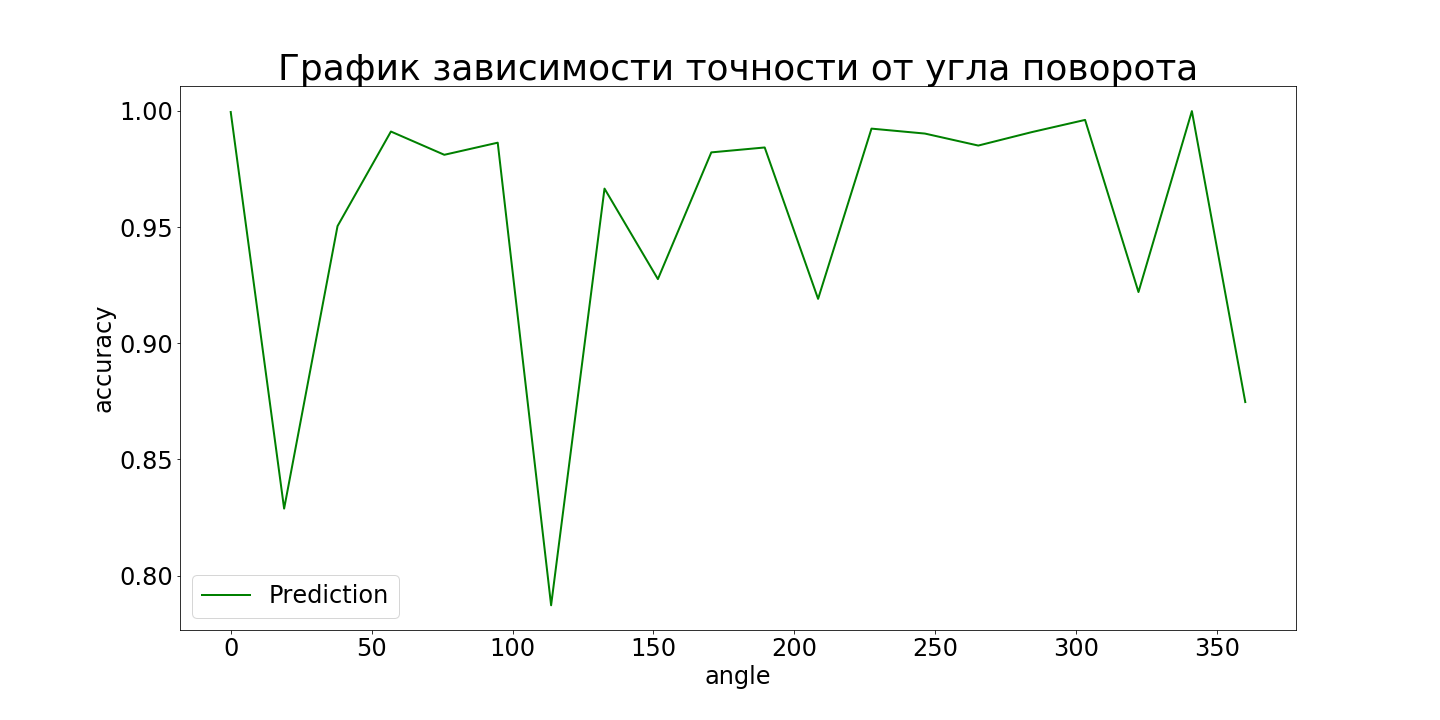
\includegraphics[width=\paperwidth]{FashionAcc.eps}}
\end{center}

\section{Выводы}

\indent\indentПроведенные тесты показывают, что нейронная сеть показывает себя очень хорошо на всем протяжении углов от $0^0$ до $360^o$. Точность редко опускается ниже $90\%$. Более низкие показатели точности возможно даже являются выбросами, связанными с малым количеством тестов.

Стоит отметить, что в рамках нашего исследования, при изучении окресности нуля, точность не падала ниже $95\%$ при вдвое большем количестве тестов.


Таким образом, можно сделать вывод, что данная нейронная сеть действительно очень хорошо справляется с отделением повернутых изображений от обычных.

\end{document}

